\chapter{Statistics}\label{Statistics}

Given data has been collected, one should apply statistical methods to analyze the data and identify assumptions about underlying properties, such as the distribution.
That is the purpose of statistical methods.

\section{Descriptive Statistics}\label{Descriptive Statistics}

\subsubsection{Mean}\label{Mean}
The mean, or average, is the sum of all values in a data set divided by the number of values. It is a measure of central tendency that provides a single value representing the center of the data.
Unlike the expected value $E$ is it used for a finite set of data points, while $E$ is a concept used for random variables and probability distributions. The mean can be seen as a specific case of the expected value when dealing with empirical data.

\subsubsection{Median}\label{Median}
The median is the middle value in a data set when the values are arranged in ascending or descending order. If the data set has an even number of observations, the median is the average of the two middle values.

\subsubsection{Mode}\label{Mode}
The mode is the value that appears most frequently in a data set. It is possible for a data set to have more than one mode if multiple values have the same highest frequency.

\subsubsection{Quantile}\label{Quantile}
Quantiles are cut points that divide the range of a data set into continuous intervals with equal probabilities. Common quantiles include quartiles (dividing data into four parts) and percentiles (dividing data into 100 parts).

\paragraph{Interquartile Range (IQR)}
The interquartile range (IQR) is the range of the middle 50\% of data, calculated as the difference between the third quartile (Q3) and the first quartile (Q1):
\begin{equation}
\text{IQR} = Q_3 - Q_1.
\end{equation}

\subsubsection{Percentile}\label{Percentile}
The percentile indicates the value below which a given percentage of observations in a group of observations falls. For example, the 20th percentile is the value below which 20\% of the observations fall. Percentiles are useful for understanding the relative standing of a value within a data set.

\emptyline
They are calculated by sorting the data set in ascending order and then finding the value below which a certain percentage of the data falls. The formula to find the k-th percentile is:
\begin{equation}
P_k = \left( \frac{k}{100} \right) (n + 1),
\end{equation}
where $P_k$ is the k-th percentile, $k$ is the desired percentile, and $n$ is the number of observations in the data set.

\subsection{Categorical Variables}\label{Categorical Variables}
\subsubsection{Nominal}\label{Nominal}
Nominal data represents categories without any intrinsic ordering. Examples include gender, race, and the presence or absence of a feature.

\subsubsection{Ordinal}\label{Ordinal}
Ordinal data represents categories with a meaningful order but no consistent difference between categories. Examples include rankings, such as class grades (A, B, C, etc.) or levels of satisfaction (satisfied, neutral, dissatisfied).

\section{Hypothesis Testing}\label{Hypothesis Testing}

\subsection{Concepts and Terminology}\label{Concepts and Terminology}

Hypothesis testing is a statistical method used to make decisions about the properties of a population based on a sample of data. It involves formulating two competing hypotheses: the null hypothesis (\(H_0\)) and the alternative hypothesis (\(H_1\) or \(H_a\)). The null hypothesis represents a statement of no effect or no difference, while the alternative hypothesis represents a statement of an effect or difference.
\begin{enumerate}
    \item [1.] Formulate the null and alternative hypotheses.
    \item [2.] Choose a significance level (\(\alpha\)), which is the probability of rejecting the null hypothesis when it is true.
    \item [3.] Collect and summarize the sample data into a test statistic.
    \item [4.] Determine the p-value, which is the probability of obtaining a test statistic at least as extreme as the one observed, assuming the null hypothesis is true.
    \item [5.] Compare the p-value to the significance level to decide whether to reject or fail to reject the null hypothesis.
\end{enumerate}
    
If the p-value is less than or equal to the significance level, the null hypothesis is rejected in favor of the alternative hypothesis. Otherwise, there is not enough evidence to reject the null hypothesis.

\subsubsection{p-value}
The p-value is the probability of obtaining a test statistic at least as extreme as the one observed, assuming the null hypothesis is true. If the p-value is less than or equal to the significance level (\(\alpha\)), the null hypothesis is rejected.

\subsubsection{Significance Level (\(\alpha\))}
The significance level (\(\alpha\)) is the probability of rejecting the null hypothesis when it is true. Common choices for \(\alpha\) are 0.05, 0.01, and 0.10.

\subsubsection{Type I and Type II Errors}
A Type I error occurs when the null hypothesis is rejected when it is true (false positive). A Type II error occurs when the null hypothesis is not rejected when it is false (false negative).

\begin{figure}[h]
    \centering
    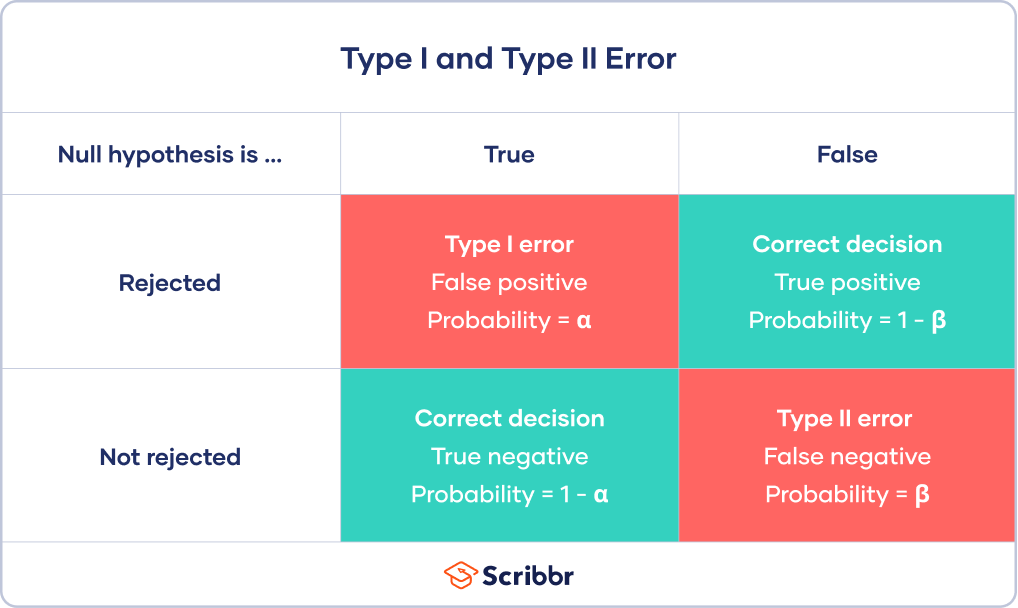
\includegraphics[width=0.6\textwidth]{../images/type-i-and-ii-error-2.png}
    \caption{Type I and Type II Errors
    {\url{https://www.scribbr.com/statistics/type-i-and-type-ii-errors/}}.}
    \label{fig:Type I and Type II Errors}
\end{figure}

\section{Test Statistic}
The test statistic is calculated from the sample data and is used to determine whether to reject the null hypothesis. The type of test statistic depends on the test being used (e.g., z-test, t-test).

\subsection{z-test}
The z-test is used for large sample sizes or when the population variance is known. It tests whether the sample mean is significantly different from the population mean.
\spacedequation{z = \frac{\bar{X} - \mu}{\sigma / \sqrt{n}},}
where $\bar{X}$ is the sample mean, $\mu$ is the population mean, $\sigma$ is the population standard deviation, and $n$ is the sample size.

\subsection{t-test}
The t-test is used for small sample sizes or when the population variance is unknown. There are different types of t-tests, including one-sample, two-sample, and paired t-tests.

\subsubsection{One-Sample t-test}
The one-sample t-test is used to determine whether the mean of a single sample is significantly different from a known or hypothesized population mean.
\spacedequation{t = \frac{\bar{X} - \mu}{s / \sqrt{n}},}
where $\bar{X}$ is the sample mean, $\mu$ is the population mean, $s$ is the sample standard deviation, and $n$ is the sample size.

\subsubsection{Two-Sample t-test}
The two-sample t-test (independent t-test) is used to compare the means of two independent samples to determine if they are significantly different from each other.
\spacedequation{t = \frac{\bar{X}_1 - \bar{X}_2}{\sqrt{\frac{s_1^2}{n_1} + \frac{s_2^2}{n_2}}},}
where $\bar{X}_1$ and $\bar{X}_2$ are the sample means, $s_1$ and $s_2$ are the sample standard deviations, and $n_1$ and $n_2$ are the sample sizes of the two groups.

\subsubsection{Paired t-test}
The paired t-test is used to compare the means of two related groups. It is often used in before-and-after studies or when the samples are matched pairs.
\spacedequation{t = \frac{\bar{D}}{s_D / \sqrt{n}},}
where $\bar{D}$ is the mean of the differences between paired observations, $s_D$ is the standard deviation of the differences, and $n$ is the number of pairs.

\subsection{Chi-square test}
\subsubsection{Chi-Square Test for Independence}
The Chi-Square Test for Independence tests if there is an association between two categorical variables. It compares the observed frequencies in each category of a contingency table to the frequencies expected if the variables were independent.
\spacedequation{\chi^2 = \sum \frac{(O_{ij} - E_{ij})^2}{E_{ij}},}
where $O_{ij}$ is the observed frequency in the $i$-th row and $j$-th column, and $E_{ij}$ is the expected frequency in the $i$-th row and $j$-th column.

\subsubsection{Chi-Square Goodness of Fit}
The Chi-Square Goodness of Fit test determines if observed frequencies match expected frequencies for a single categorical variable. It assesses how well the observed distribution of data fits with the distribution expected under a specific hypothesis.
\spacedequation{\chi^2 = \sum \frac{(O_i - E_i)^2}{E_i},}
where $O_i$ is the observed frequency and $E_i$ is the expected frequency for the $i$-th category.

\subsection{ANOVA (Analysis of Variance)}
ANOVA is used to compare means among three or more groups to see if at least one group mean is different from the others. It analyzes the variance within groups and between groups.

\subsubsection{One-Way ANOVA}
One-way ANOVA is used when there is one independent variable with multiple levels (groups). It tests whether there are any statistically significant differences between the means of three or more independent (unrelated) groups.
\spacedequation{F = \frac{\text{variance between groups}}{\text{variance within groups}}.}

\subsubsection{Two-Way ANOVA}
Two-way ANOVA is used when there are two independent variables. It tests the effect of two factors simultaneously and also examines the interaction between the two factors.
\spacedequation{F = \frac{\text{variance due to factor A, factor B, and interaction}}{\text{variance within groups}}.}

\subsection{F-Test}
The F-test is used to compare the variances of two groups to determine if they are significantly different. It is based on the ratio of the two sample variances.
\begin{equation}
F = \frac{s_1^2}{s_2^2},
\end{equation}
where $s_1^2$ and $s_2^2$ are the sample variances of the two groups.

\subsection{Levene’s Test}
Levene’s Test is used to check for equality of variances across groups. It is more robust to departures from normality than the F-test. The test statistic is calculated as:
\begin{equation}
W = \frac{(N - k)}{(k - 1)} \frac{\sum_{i=1}^k N_i (Z_{i\cdot} - Z_{\cdot\cdot})^2}{\sum_{i=1}^k \sum_{j=1}^{N_i} (Z_{ij} - Z_{i\cdot})^2},
\end{equation}
where $Z_{ij} = |Y_{ij} - \bar{Y}_i|$, $Y_{ij}$ is the value of the $j$-th case in the $i$-th group, $\bar{Y}_i$ is the mean of the $i$-th group, $Z_{i\cdot}$ is the mean of the $Z_{ij}$ in the $i$-th group, and $Z_{\cdot\cdot}$ is the mean of all $Z_{ij}$.


\subsection{Pearson Correlation Coefficient}\label{Pearson Correlation Coefficient}
In statistical analysis, the relationship between the independent and dependent variables can be analyzed using various methods such as correlation and regression analysis. The correlation coefficient $r$ measures the strength and direction of the linear relationship between two variables:
\spacedequation{r = \frac{\sum (X_i - \bar{X})(Y_i - \bar{Y})}{\sqrt{\sum (X_i - \bar{X})^2 \sum (Y_i - \bar{Y})^2}},}
where $X_i$ and $Y_i$ are the individual sample points, and $\bar{X}$ and $\bar{Y}$ are the means of $X$ and $Y$ respectively.

\emptyline
These are basic statistical methods not needing much computational power. However, a layer deeper statisticians build models to describe their observations.  
Because it is beyond the scope of this chapter, it will not discuss it here.